\section{Lecture 06-03-2018}

\begin{enumerate}
	\item Impedance matching
	\item L network
	\item Pi network
	\item T network
\end{enumerate}

\noindent\fbox{\parbox{\textwidth}{
	\begin{itemize}
		\item \textbf{Curriculum:} CB, Ch 4 p. 63-72
		\item \textbf{Tasks:} Lektion 4-1, Lektion 4-2, Lektion 4-3
	\end{itemize}
}} \vspace{3mm}

\noindent\textit{Impedance matching is often necessary in the design of RF circuitry to provide the maximum possible transfer of power	between a source and its load.}

\subsection{L network}
\begin{itemize}
	\item 4 possible combinations of placement of L and C components.
	\begin{itemize}
		\item 2 combinations that result in a lowpass configuration.
		\item 2 combinations that result in a highpass configuration.
	\end{itemize}
\end{itemize}

\subsubsection{Analysis}
\begin{itemize}
	\item Determine what the load impedance actually looks
	like when the capacitor is placed across the load resistor.
\end{itemize}

\begin{equation}
Z = \dfrac{X_C R_L}{X_C+R_L}
\end{equation}

\begin{itemize}
	\item The parallel combination of the capacitor and resistor looks like an impedance in series.
	\item To complete the impedance match to source resistance is to add an equal and opposite reactance in series.
	\item The addition of the inductor causes cancellation of the capacitor leaving only an apparent load resistor.
	\begin{itemize}
		\item The shunt component of the impedance-matching network is to transform a larger impedance downto a smaller value with a real part equal to the real part of the other terminating impedance.
		\item The series impedance-matching element then resonates with or cancels any reactive component present, thus leaving the source driving an apparently equal load for optimum power transfer.
	\end{itemize}
\end{itemize}


\begin{figure} [H]
	\centering
	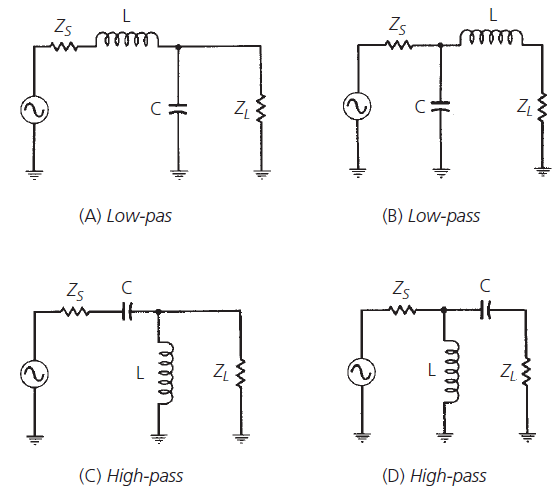
\includegraphics[width=0.8\linewidth]{graphics/26.png}
	\caption{L network.}
	\label{fig:26}
\end{figure}

\newpage\subsubsection{Design}

\begin{itemize}
	\item $X_p$ and $X_s$ may be either capacitive or inductive reactance but each must be of the opposite type. Once $X_p$ is chosen as a capacitor, for example, $X_s$ must be an inductor, and vice versa.
\end{itemize}

\begin{equation}
Q_s = Q_p = \sqrt{\dfrac{R_p}{R_s}-1}
\end{equation}

\begin{equation}
Q_s = \dfrac{X_s}{R_s}
\end{equation}

\begin{equation}
Q_p = \dfrac{R_p}{X_p}
\end{equation}

\begin{description}
	\item[$Q_s$] Q of the series leg
	\item[$Q_p$] Q of the shunt leg
	\item[$R_p$] shunt resistance
	\item[$X_p$] shunt reactance
	\item[$R_s$] series resistance
	\item[$X_s$] series reactance
\end{description}

\subsubsection{Complex loads}
Two basic approaches in handling complex impedances.
\begin{itemize}
	\item Absorption
	\begin{itemize}
		\item Absorb any stray reactances into the impedance-matching network itself.
		\item Done through placement of each matching element such that element capacitors are placed in parallel with stray capacitances.
		\item Element inductors are placed in series with any stray inductances. 
		\item Stray component values are subtracted from the calculated element
		values, leaving new element values (C', L'), smaller than the calculated element values.
	\end{itemize}
	\item Resonance
	\begin{itemize}
		\item Resonate any stray reactance with an	equal and opposite reactance at the frequency of interest.
	\end{itemize}
\end{itemize}

\subsection{Pi network}
\textit{Two "back-to-back" L networks that are both configured to match the load and
	the source to an invisible or "virtual" resistance located at the junction between the two networks.}

\begin{figure} [H]
	\centering
	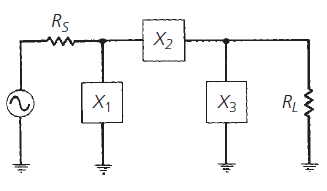
\includegraphics[width=0.6\linewidth]{graphics/27.png}
	\caption{Three element Pi network.}
	\label{fig:27}
\end{figure}

\begin{itemize}
	\item The negative signs for $-X_{s1}$ and $-X_{s2}$ is symbolic.
	\item Used to indicate that the $X_s$ values are the opposite type of reactance from $X_{p1}$ and $X_{p2}$.
\end{itemize}

\begin{figure} [H]
	\centering
	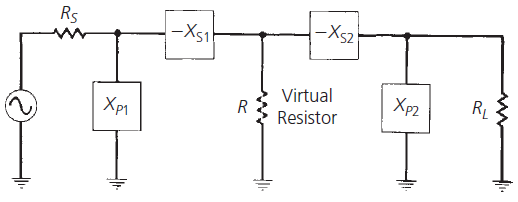
\includegraphics[width=0.8\linewidth]{graphics/29.png}
	\caption{Pi network shown as two back-to-back L networks.}
	\label{fig:29}
\end{figure}

\subsubsection{Design}
\begin{itemize}
	\item The virtual resistance (\textit{R}) must be smaller than either $R_s$ or $R_L$.
	\item Most of the time, \textit{R} is defined by the desired loaded \textit{Q} of the
	circuit that you specify.
\end{itemize}

\begin{equation}
Q = \sqrt{\dfrac{R}{R_{small}}-1}
\end{equation}


\subsection{T network}
\textit{The T network is often used to match two low-valued impedances when a high-Q arrangement is needed.}

\begin{figure} [H]
	\centering
	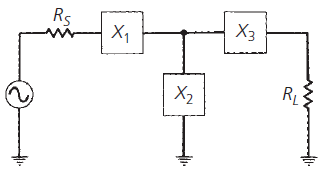
\includegraphics[width=0.6\linewidth]{graphics/28.png}
	\caption{Three element T network.}
	\label{fig:28}
\end{figure}

\noindent\textit{The Pi and T networks are great for narrow-band matching networks.\\
What if an impedance match is required over a fairly broad range of frequencies?}

\begin{itemize}
	\item Two series-connected L sections rather than the back-to-back configuration
	of the Pi and T networks.
	\begin{itemize}
		\item Value of the virtual resistor (R) must be larger than the smallest termination impedance and smaller than the largest termination
		impedance.
	\end{itemize}
	\item Maximum bandwidth (minimum Q) available:
\end{itemize}

\begin{equation}
R = \sqrt{R_S R_L}
\end{equation}

\begin{equation}
Q = \sqrt{\dfrac{R}{R_{smaller}-1}}= \sqrt{\dfrac{R_{larger}}{R}-1}
\end{equation}

\begin{description}
	\item[$R$] virtual resistance
	\item[$R_{smaller}$] smallest terminating resistance
	\item[$R_{larger}$] largest terminating resistance
\end{description}

\noindent\textit{If even wider bandwidths are needed, more L networks may be	cascaded with virtual resistances between each network.}
\begin{equation}
\dfrac{R_1}{R_{smaller}} = \dfrac{R_2}{R_1}= \dfrac{R_3}{R_2} ... = \dfrac{R_{larger}}{R_n}
\end{equation}

\begin{figure} [H]
	\centering
	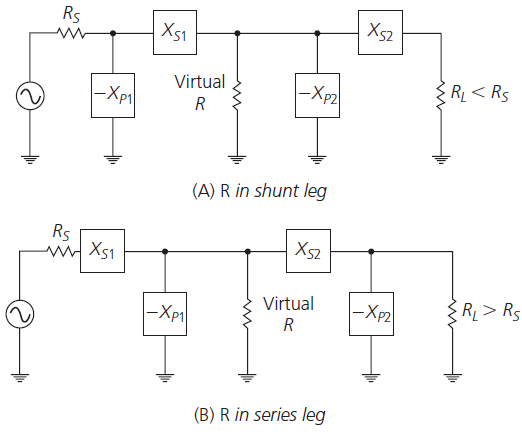
\includegraphics[width=0.8\linewidth]{graphics/30.png}
	\caption{Two series-connected L networks for lower Q applications.}
	\label{fig:30}
\end{figure}

\noindent\fbox{\parbox{\textwidth}{
		\begin{itemize}
			\item \textcolor{red}{Series element should be placed at  lowest impedance.}
			\item \textcolor{red}{Parallel element should be placed at highest impedance.} 
		\end{itemize}	
}} \vspace{3mm}